%% Use the hmcposter class with the thesis document-class option.
\documentclass[thesis]{hmcposter}
\usepackage{graphicx} 
\usepackage{natbib}
\usepackage{booktabs}
\usepackage{subfig} 
\usepackage{amsmath} 
\usepackage{textcomp} 
\usepackage{url}  


\usepackage{hyperref}
\usepackage{cite} 
\usepackage[utf8]{inputenc}
\usepackage[portuguese]{babel}

%\usepackage{biblatex}  
%\bibliography{refs}
 
%% Author of the thesis.
\author{Ayrton Denner da Silva Amaral}

%% The year of your thesis poster's creation.
\posteryear{2017}

%% Thesis Title.
\title{Predição de tendência de apostas em bolsas esportivas}

%% The name of the class for which the poster was created.
%% Generally we see posters for thesis and Clinic, but sometimes
%% other classes require or allow the creation of posters to
%% communicate the results of a project.
%% 
%% Use the format Math nnn: Class Title.
\class{Algoritmos de Reconhecimento de Padrões}

%% Advisor(s) name or names.  Separate with \and.
\advisor{Gustavo Teodoro Laureano\and Anderson da Silva Soares}

%% Reader(s) name or names.  Separate with \and.
%\reader{Gustavo Teodoro Laureano \and Anderson da Silva Soares}

%% Optional -- if you are especially concerned about intellectual
%% property issues (maybe you have some potentially patentable
%% material in your thesis), you can use the \copyrightholder
%% command to supply a name for a copyright holder for your
%% poster.  Note that under U.S. law, all works are under
%% copyright from the moment of creation; the copyright statement
%% is merely making your claim obvious.
%%
%% This command is also useful if you are sharing copyright of the
%% poster with someone else (e.g., a student collaborator, your
%% advisor, an organization).
%%
%\copyrightholder{Claire~M. Connelly and the Department of Mathematics, Harvey Mudd College}


%% Define the \BibTeX command, used in our example document.
\providecommand{\bibtex}{{\rmfamily B\kern-.05em%
    \textsc{i\kern-.025em b}\kern-.08em%
    T\kern-.1667em\lower.7ex\hbox{E}\kern-.125emX}}


\pagestyle{fancy}

\begin{document}

\begin{poster}

\section{Introdução}
% Note that we're not labeling sections because you shouldn't be
% doing a lot of referring back and forth in your poster---let the
% interested folks read your thesis or Clinic report, or ask
% questions.

Atualmente, a Betfair é a maior bolsa esportiva do mundo.
Com mais de 15 anos em atividade e 4 milhões de usuários cadastrados, movimenta aproximadamente £400 milhões anualmente. Na Figura~\ref{fig:betfair-print}, podemos ver uma imagem do site.

\begin{figure}
\begin{center}
\fbox{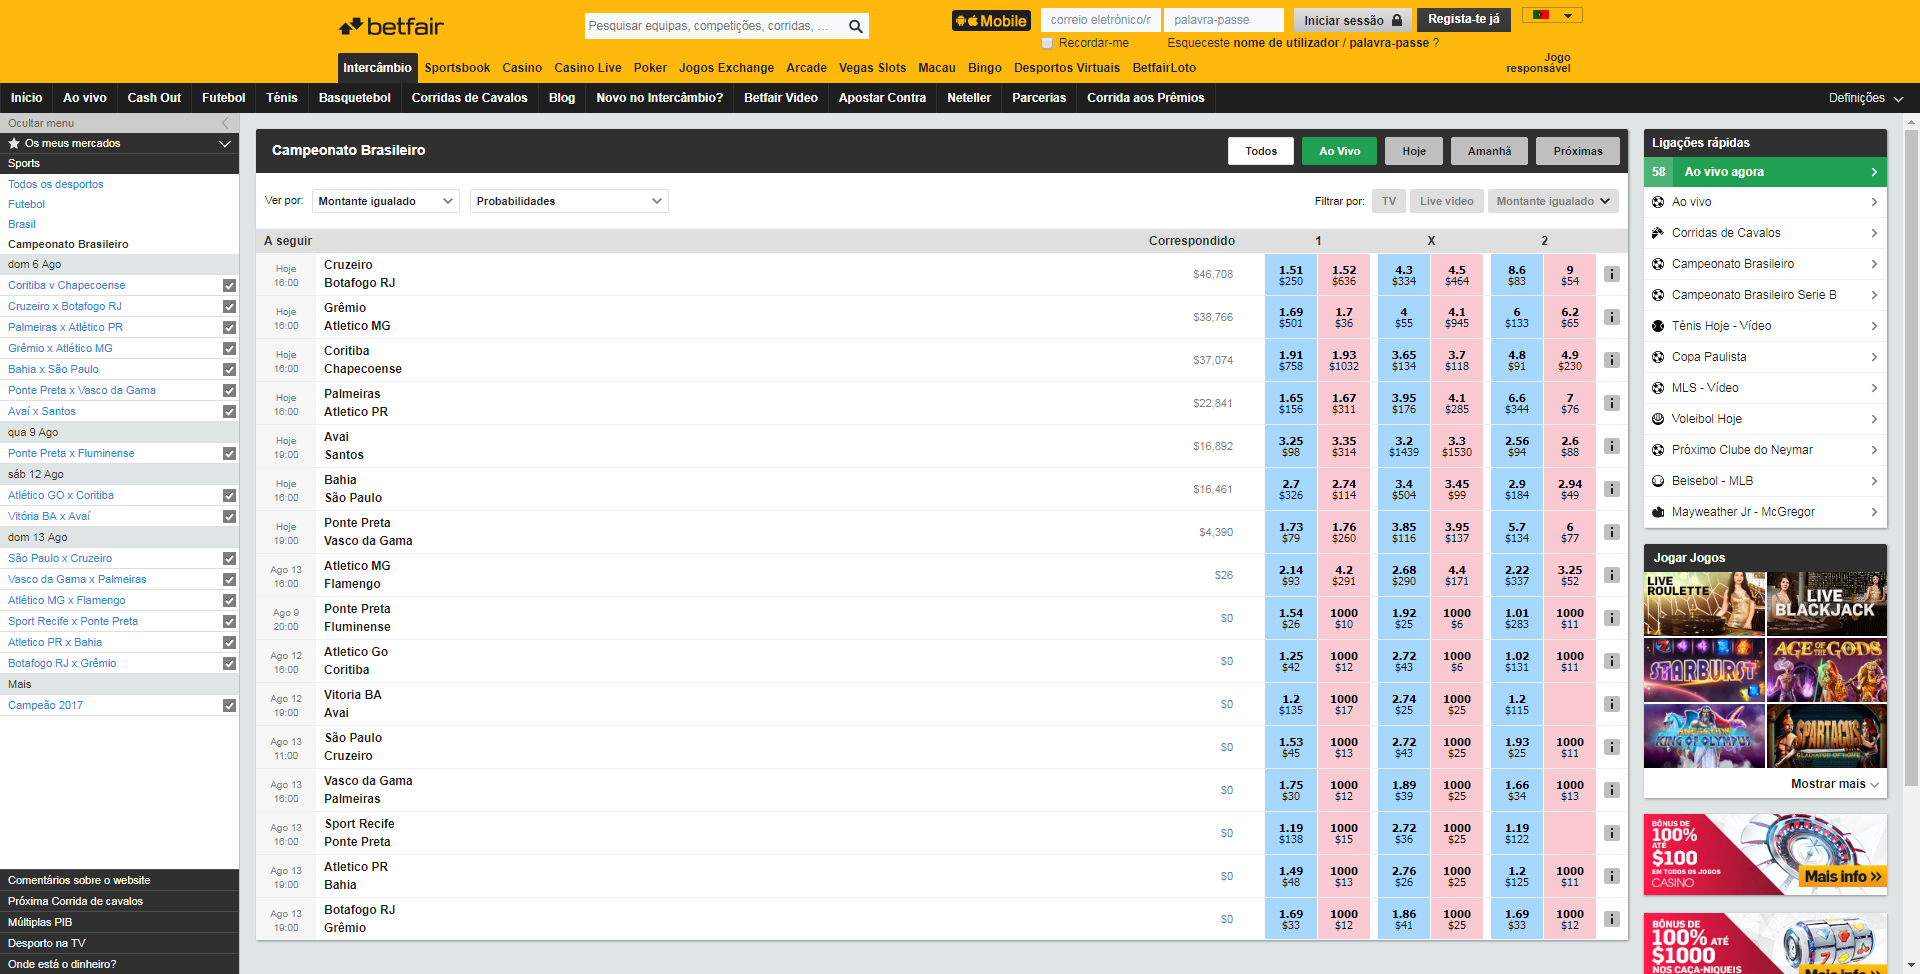
\includegraphics[width=10in]{screencapture-betfair-exchange-plus-football-competition-13-1502038892160.png}}
\caption{Imagem do site Betfair}%
\label{fig:betfair-print}
\end{center}
\end{figure}

Nesse projeto, buscamos a predição de qual categoria receberá um maior número de apostas em um período observado, seja o time da casa, time visitante ou opção de empate, analisando especificadamente os jogos da Série A do Campeonato Brasileiro de 2016.

\section{Materiais e métodos}%

Para o desenvolvimento do projeto, foram tomadas uma sequência de etapas para o uso dos dados:

\begin{itemize}
\item Foram utilizadas a biblioteca \emph{scikit-learn} para os algoritmos de aprendizado de máquina, e a biblioteca \emph{NumPy} para manipulação de vetores e matrizes, ambas utilizando a linguagem Python.
\item Também utilizamos a suíte \emph{Weka} para aplicação dos algoritmos de aprendizado de máquina.
\item Analisamos os dados oferecidos pela Betfair por todo o ano de 2016, em uma base de aproximadamente 55 milhões de linhas.
\item Ao aglutinarmos os dados de uma mesma partida, atingimos o número de 379 linhas, a mesma quantidade de jogos no ano de 2016.
\item Também foi necessário um pré-processamento dos dados oferecidos, como transformar datas e nome dos times em números (esse último via técnica de \emph{one-hot encoding}), e adicionar a quantidade de vitórias de cada time nos últimos 5 jogos.
\item No final de todas essas etapas e com todos os dados preparados para o processamento, finalmente aplicamos os algoritmos de aprendizado de máquina de categorização aos valores obtidos.
\end{itemize}

\section{Resultados}%

Após filtrarmos e trabalharmos com os dados restantes, os primeiros resultados obtidos foram acerca da eficácia dos algoritmos preverem os resultados como um todo, exibidos na Figura~\ref{fig:algoritmo-total}:

\begin{figure}
\begin{center}
\fbox{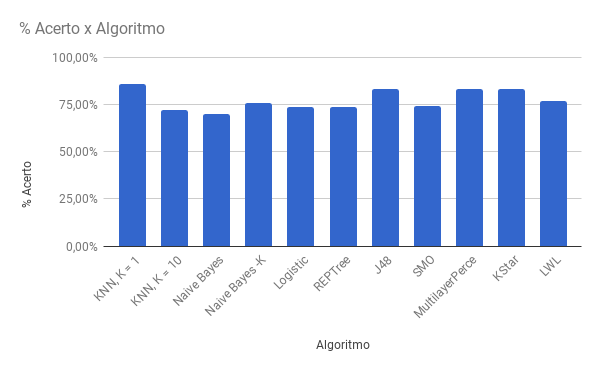
\includegraphics[width=10in]{imagens_algoritmo/algoritmo_total.png}}
\caption{Porcentagem de acerto dos algoritmos para todos os resultados}%
\label{fig:algoritmo-total}
\end{center}
\end{figure}

Porém, esses resultados não são suficientes. Ainda que os algoritmos tenham bons resultados com todas as categorias, é necessário especificar a eficácia de cada algoritmo com cada categoria possível de apostas (time da casa, time visitante ou empate). Essa diferença se faz visível no próximo gráfico da Figura~\ref{fig:algoritmo-categoria}:

\begin{figure}
\begin{center}
\fbox{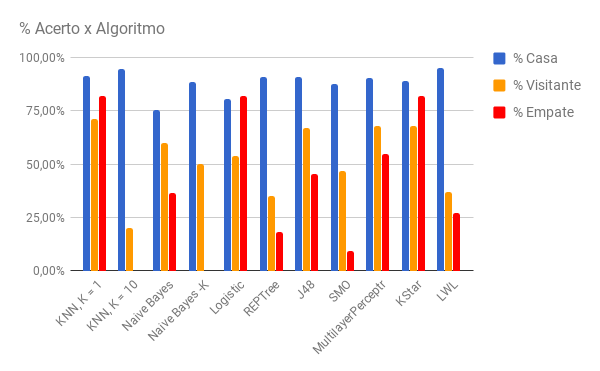
\includegraphics[width=10in]{imagens_algoritmo/algoritmo_categoria.png}}
\caption{Porcentagem de acerto dos algoritmos para resultados de cada categoria}%
\label{fig:algoritmo-categoria}
\end{center}
\end{figure}

Outro valor que também podemos utilizar para análise é o chamado Coeficiente de Kappa, que mede a concordância entre os valores da classificação apresentada, apresentado na Figura~\ref{fig:algoritmo-kappa}:

\begin{figure}
\begin{center}
\fbox{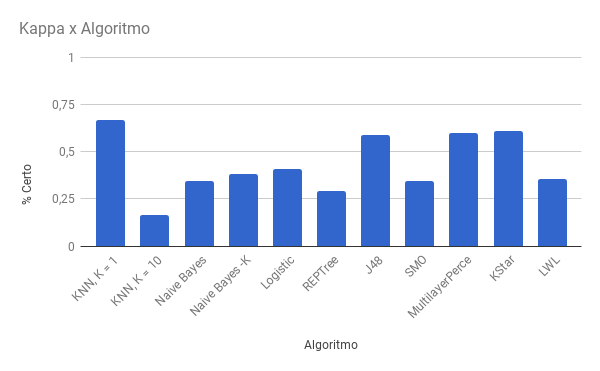
\includegraphics[width=10in]{imagens_algoritmo/algoritmo_kappa.png}}
\caption{Porcentagem do Coeficiente de Kappa para cada algoritmo utilizado}%
\label{fig:algoritmo-kappa}
\end{center}
\end{figure}

\section{Conclusões}

Ao final dessas análises, fica visível que um valor alto de acerto para o total de dados não é necessariamente um resultado bem-sucedido, podendo ser apenas um falso positivo que ignora a situação das categorias em específico.

O próximo passo do nosso trabalho de predição será buscar a quantificação de apostas em cada opção das bolsas esportivas. Ou seja, iremos buscar quantas apostas cada opção receberá, ao invés de apenas indicar qual opção receberá mais apostas.

Como forma de buscar resultados mais eficazes, será necessário uma busca por bases mais completas em relação a eventos esportivos, com outros dados e estatísticas que possam melhor agregar no resultado final.

\section{Agradecimentos}

Por primeiro, gostaria de agradecer ao Instituto de Informática da Universidade Federal de Goiás, por oferecer o espaço para essa apresentação, além de ofertar essas e outras matérias relevantes para área.

Por segundo, gostaria de agradecer aos professores Anderson Soares e Gustavo Laureano, que ministraram a disciplina de Algoritmos de Reconhecimento de Padrões, e que junto com os outros colegas da turma, também ajudaram na construção dos trabalhos e no entendimento do conteúdo apresentado.

Por último, gostaria de agradecer a aqueles que reservaram um pouco do seu tempo para prestigiar essa apresentação.

\section{Para maiores informações}

\begin{itemize}
\item Email para contato: \url{ayrtondenner_2013@hotmail.com}
\item Link para repositório no Github do poster: \url{https://github.com/ayrtondenner/ARP-2017-1/tree/master/Poster%20-%20Landscape}
\item Seção da Betfair para jogos da Série A do Campeonato Brasileiro \url{https://www.betfair.com/exchange/plus/football/competition/13}
\item Lista com dados históricos da Betfair: \url{http://data.betfair.com/}
\end{itemize}

\end{poster}

\end{document}